\section{Data}
    
    The full TCGA-BRCA RNA-sequencing dataset was downloaded from the NCI's GDC data portal \cite{gdc2016} using R/Bioconductor package TCGAbiolinks v2.8.13
\cite{Colaprico2016}. The overview of available breast cancer RNA-seq samples collected by the TCGA research network is displayed in Table \ref{table:full}. 

     %   TABLE 2.1
     
            \begin{table}[!htbp]
            \centering
            \caption{Overview of RNA-Seq samples in the TCGA-BRCA dataset. Top row: all available samples, Bottom row: samples used in the project.}
            \label{table:full}          
            \begin{tabular}{cc|c|c|c}
            \multicolumn{1}{l}{} & \textbf{Samples} & \textbf{Tumour} & \textbf{Normal} & \textbf{Metastasis} \\ \cline{2-5} 
            \multicolumn{1}{c|}{\textbf{\begin{tabular}[c]{@{}c@{}}Full\\  dataset\end{tabular}}} & 1212 & \begin{tabular}[c]{@{}c@{}}1093\\ (F: 1081, M: 12)\end{tabular} & \begin{tabular}[c]{@{}c@{}}112\\ (F: 112, M :0)\end{tabular} & \multicolumn{1}{c|}{\begin{tabular}[c]{@{}c@{}}7\\ (F: 7, M: 0)\end{tabular}} \\ \hline
            \multicolumn{1}{c|}{\textbf{\begin{tabular}[c]{@{}c@{}}Final\\  dataset\end{tabular}}} & 969 & F:857 & F:112 & \multicolumn{1}{l|}{} \\ \cline{2-5} 
            \end{tabular}
            \end{table}
                 

    The full dataset has been reduced to include samples that matched three criteria: \textbf{ i)} samples from female patients only (to reduce biological variation coming from gender) \textbf{ii)} samples that have been manually curated for their classifications \textbf{iii)} samples that are provided with sufficient metadata to benefit exploratory analysis. Only primary tumour and normal samples were included in the analysis.
    
    
    \subsection{Samples Annotation}
    Morphological and stage annotation of samples included in the analysis was curated by the members of CBL group and the collaborators from other groups at DCRC. Table \ref{table:morphstage} shows the number of samples that were represented in the morphological groups and stages in the final dataset. 
    
    
     %   TABLE 2.2
            \begin{table}[!htbp]
            \centering
            \caption{The number of samples in each morphology type and stage in the final datset. 'Stage X' is unknown/unidentifiable stage. 'Other morphologies' comprises various other mophologies that are represented by only a few samples.}
            \label{table:morphstage}
            \begin{tabular}{lccllclc}
            \multicolumn{1}{c}{\textbf{Morphology}} & \textit{\begin{tabular}[c]{@{}c@{}}ICD-O-3 \\ code\end{tabular}} & \textbf{} &  &  & \textbf{} & \multicolumn{1}{c}{\textbf{Stage}} & \textbf{} \\ \cline{1-3} \cline{7-8} 
            \multicolumn{1}{|l|}{Invasive Lobular Carcinoma} & \multicolumn{1}{c|}{8520/3} & \multicolumn{1}{c|}{143} &  &  & \multicolumn{1}{c|}{} & \multicolumn{1}{l|}{stage 1} & \multicolumn{1}{c|}{148} \\ \cline{1-3} \cline{7-8} 
            \multicolumn{1}{|l|}{Invasive Ductal Carcinoma} & \multicolumn{1}{c|}{8500/3} & \multicolumn{1}{c|}{644} &  &  & \multicolumn{1}{c|}{} & \multicolumn{1}{l|}{stage 2} & \multicolumn{1}{c|}{481} \\ \cline{1-3} \cline{7-8} 
            \multicolumn{1}{|l|}{Ductal and Lobular \textit{in situ} Carcinoma} & \multicolumn{1}{c|}{8522/3} & \multicolumn{1}{c|}{24} &  &  & \multicolumn{1}{c|}{} & \multicolumn{1}{l|}{stage 3} & \multicolumn{1}{c|}{195} \\ \cline{1-3} \cline{7-8} 
            \multicolumn{1}{|l|}{Metaplastic carcinoma} & \multicolumn{1}{c|}{8575/3} & \multicolumn{1}{c|}{7} &  &  & \multicolumn{1}{c|}{} & \multicolumn{1}{l|}{stage 4} & \multicolumn{1}{c|}{12} \\ \cline{1-3} \cline{7-8} 
            \multicolumn{1}{|l|}{Mucinous carcinoma} & \multicolumn{1}{c|}{8480/3} & \multicolumn{1}{c|}{12} &  &  & \multicolumn{1}{c|}{} & \multicolumn{1}{l|}{stage X} & \multicolumn{1}{c|}{21} \\ \cline{1-3} \cline{7-8} 
            \multicolumn{1}{|l|}{Other morphologies} & \multicolumn{1}{l|}{} & \multicolumn{1}{c|}{27} &  &  &  & \multicolumn{1}{c}{} &  \\ \cline{1-3}
            \end{tabular}
            \end{table}
    
 

    All samples in the final dataset were annotated with clinical data, which included PAM50 molecular subtype, patient age subgroup, race/ethnicity, menopause status, tumour grade, nodal involvement, metastasis status, year sample was taken, and tissue source site. The annotations extracted with TCGAbiolinks were integrated with further information from the work by Rahman \textit{et al. }\cite{RahmanAlternativeResults} on reprocessing TCGA data. 
    The original set of PAM50 subtype annotations available for TCGA data that was obtained by a large TCGA-BRCA study in 2012 \cite{CancerGenomeAtlasNetwork2012ComprehensiveTumours}, was further complemented with the additional subtype labels for the previously unclassified samples from a recent TCGA-BRCA study by Ciriello \textit{et al.} in 2015 \cite{Ciriello2015ComprehensiveCancer}. A small minority of samples that had discrepancies in labels between the two studies were omitted in this project.  Table \ref{table:pam50counts} shows the sample counts for each PAM50 subtype. 
    
    
     %   TABLE 2.3   
                \begin{table}[!htbp]
                \centering
                \caption{The number of samples in each PAM50 molecular subtype in the final dataset.}
                \label{table:pam50counts}
                \begin{tabular}{ll}
                \multicolumn{1}{c}{\textbf{PAM50}} &  \\ \hline
                \multicolumn{1}{|l|}{Luminal A} & \multicolumn{1}{l|}{420} \\ \hline
                \multicolumn{1}{|l|}{Luminal B} & \multicolumn{1}{l|}{183} \\ \hline
                \multicolumn{1}{|l|}{Basal-like} & \multicolumn{1}{l|}{153} \\ \hline
                \multicolumn{1}{|l|}{HER2-enriched} & \multicolumn{1}{l|}{75} \\ \hline
                \multicolumn{1}{|l|}{Normal-like} & \multicolumn{1}{l|}{26} \\ \hline
                \end{tabular}
                \end{table}
                

    
    
     \subsection{Genes Annotation}   
    A curated collection of autophagy-related gene lists was provided by experts in the field at DCRC (in the Cell Death and Metabolism and Cell Stress and Survival Units). Table \ref{table:autophagy} shows the functional groups that autophagy-related genes are managed by. The autophagy core genes and as well as transcription factors are of the most interest. 
    
     %   TABLE 2.4
    
            \begin{table}[!htbp]
            \centering
            \caption{Autophagy-related genes functional groups. The numbers are reported for the dataset after pre-processing with TCGAbiolinks. Some genes are present in more that one group. }
            \label{table:autophagy}
            \begin{tabular}{l|c}
            \small
            \textbf{Functional Group} & \multicolumn{1}{l}{\textbf{Number of genes}} \\ \hline
            Autophagy core & 156 \\ \hline
            Transcription factors & 101 \\ \hline
            Lipid & 33 \\ \hline
            Phosphatidyl & 40 \\ \hline
            Endo and exosomes & 132 \\ \hline
            Transport & 216 \\ \hline
            RABs and effectors & 131 \\ \hline
            Docking and fusion & 14 \\ \hline
            Mitophagy & 65 \\ \hline
            Receptors and ligands & 66 \\ \hline
            mTOR induction & 138 \\ \hline
            Lysogenesis induction & 62 \\ \hline
            Lysosome & 218 \\ \hline
            \multicolumn{1}{c|}{\textit{Total}} & \textit{1112}
            \end{tabular}
            \end{table}
            
            
            
            
    \subsection{Extraction and Preparation}
    
    The TCGA-BRCA RNA-seq data was generated using \textit{Illumina HiSeq 2000 RNA Sequencing Version 2 analysis} platform and quantified at University of North Carolina (UNC) Center for Bioinformatics for the TCGA project \cite{UniversityofNorthCarolinaUNCCenterforBioinfromatics2013TCGAData}. The quantification pipeline included  using Mapsplice v12.07 \cite{wang2010mapsplice} for mapping the data to reference genome (GRCh37/hg19), RSEM v1.1.13 \cite{li2011rsem} for transcript quantification \cite{UniversityofNorthCarolinaUNCCenterforBioinfromatics2013TCGAData}. 

    Level 3 legacy TCGA-BRCA gene expression dataset was downloaded from the GDC portal and prepared using the TCGAbiolinks preprocessing pipeline. The pipeline contains integrated functions from the EDASeq package \cite{risso2011gc} for within-lane normalisation procedures to adjust for GC-content and gene length effects on read counts, as well as between-lane normalisation method to adjust for distributional differences between lanes (e.g. sequencing depth), such as quantile normalisation \cite{Colaprico2016, PapaleoTCGAPackages}. 
    In this project, the dataset was normalised for GC-content and filtered with with quantile cut-off of 0.10. The pipeline transforms the data into a '\textit{SummarizedExperiment}' \cite{Huber2015OrchestratingBioconductor} object (counts table), with genes and samples as rows and columns, respectively. 
    
        
    After data pre-processing and selecting the samples with sufficient clinical information, the final dataset included 857 tumour and 112 normal samples, and  the gene expression matrix was reduced to 17372 genes. Figure \ref{fig:workflow} aims to summarise the data flow from the original dataset thorough to the downstream analysis. The next section will describe the further processing applied to the data prior to analysis. 
    
    
       % workflow
            \begin{figure}[h]
            \centering
            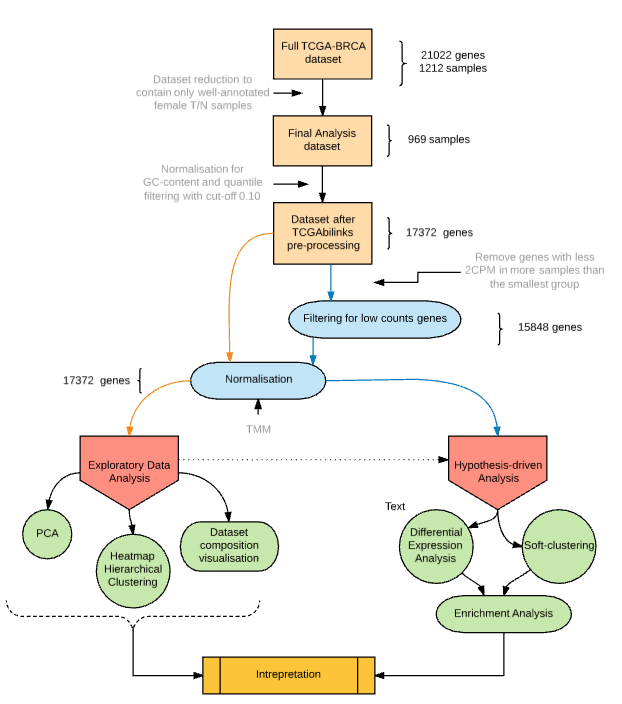
\includegraphics[scale=0.8]{analysis_workflow_test.png}
            \caption{Project workflow overview. Several pre-processing and filtering steps reduce the number of samples and genes in the original dataset prior to Exploratory and Hypothesis-driven data analyses. The data is normalised so that samples can be more appropriately compared. Exploratory Analysis guides Hypothesis-driven Analysis. The observations from both are used for biological interpretation. }
            \label{fig:workflow}
            \end{figure} 
    
    \subsection{Filtering and Normalisation}
    
   Throughout different parts of analysis the counts data is stored in a simple list-based data object \texttt{DGEList} from R package \texttt{edgeR} \cite{Robinson2010EdgeR:Data}, which also contains sample annotation and library size information. 

    For differential expression and related analyses, gene expression is not considered as raw counts, because library sizes (total number of mapped reads) differ and result in higher counts. Therefore, it is a common practice to transform raw counts onto a scale that accounts for such library size differences \cite{law2016rna}. Popular transformations include (log2-)counts per million (log-CPM/CPM), and reads/fragments per kilobase of transcript per million (RPKM/FPKM). CPM is a simple measure of read abundance that can be compared across libraries of different sizes, i.e. it is relative change in expression \cite{Law2014}. Standardising further by gene length gives RPKM, which is an absolute expression. Data in the form of CPM, log-CPM, and RPKM will be used for different parts of analysis in this project. 
    
    Prior to the analysis it is important to filter out genes with very low counts across all libraries, as they provide more noise than evidence, e.g. for differential expression. Genes that are not expressed at a biologically meaningful level in any condition should be discarded to reduce the subset of genes to those that are of interest, and to minimise the number of tests carried out downstream. In this project, filtering was done based on CPM to account for library sizes. The selected cut-off for keeping the genes was guided by the mean-variance plot produced by \texttt{voom} function (discussed in Section 3.3.1.2). The genes with at least 2 CPM expression in at least 19 samples passed the threshold and were used in the analysis.
    
    After filtering, the samples have to be normalised before they can be compared. This step is required to ensure that the expression distribution of samples is similar across the entire experiment \cite{Robinson2010}. In this project, normalisation by the method of trimmed mean of M-values (TMM) \cite{RobinsonAData} was performed using the \texttt{calcNormFactors} function in \texttt{edgeR} to rescale the library sizes to take into account differences in RNA-composition. In this way, the effective library size replaces the original library size in all downstream analyses. 
    
    Normalisation adjusts global properties of measurements for individual samples so that they can be more appropriately compared, and is now a standard practice in analysis of gene expression data. However, normalisation does not remove batch effects, which can affect subsets of genes in different ways. The topic of batch effects in gene expression data will discussed in Section 3.2.3. 

    
             
   
    
    
   
\newpage    
\section{Exploratory analysis methods}
    
    Exploratory data analysis (EDA) is an essential step in working with large publicly available datasets, such as the TCGA-BRCA in this project. Application of exploratory analysis to transcriptomics data can be a means of visualising the global structure of the data, and also serve three major roles: 
    
    \begin{enumerate}
      \item Discover patterns and spot outliers/abnormalities
      \item Frame the hypothesis
      \item Check assumptions 
    \end{enumerate}
    
    After normalisation described in the previous section, the data is ready to be analysed.  Metadata available for samples is to be rigorously explored to maximise the insight into the dataset and extract important features.
    
    Principal component analysis and clustering (as part of a heatmap and not) are the most commonly used exploratory tools. The underlying statistics and algorithms available for the calculations involved in PCA and clustering dendogram generation are fundamentally the same for the available packages in R/Bioconductor. 
    This section will present a general introduction to PCA and clustering, and provide simple examples of use.

    
    \subsection{Principal Component Analysis}
    
    Principal component analysis (PCA) is a method that linearly transforms a multivariate dataset into a set of uncorrelated variables ordered in descending manner by the variance explained \cite{jolliffe2002principal}. In this way, the first few principal components (PCs) often explain the largest amount of the variation in the data. PCA results can be visualised in a 2D scatter plot, where $x$ and $y$ axes are the selected principal components. The samples are projected onto the 2D plane such that they spread out in the two directions that capture the most of the variance across samples \cite{Love2016RNA-SeqApproved}. 
    In a PCA 2D scatter plot, each data point represents a sample, which allows visualisation of sample clustering and dataset structure.  The relationship between two samples is reflected by the distance between corresponding dots in the plot. Therefore, the more similar gene expression profiles are, the closer the data points are.    
   
    Figure \ref{fig:pcamethod} shows an example of separation of transcriptional profiles of cancer (pink) and normal (blue) samples. The primary source of variation (PC1) accounts for 11\% of the total variation in the data. The second principal component (PC2) accounts for 8.6\% of the total variation in the data. 
    Here, and throughout the project, PCA was performed using the R function \texttt{prcomp()}, the plots were generated with R package \texttt{ggplot2} \cite{ggplot2}.
    
        % PCA plot 
            \begin{figure}[!h]
            \centering
            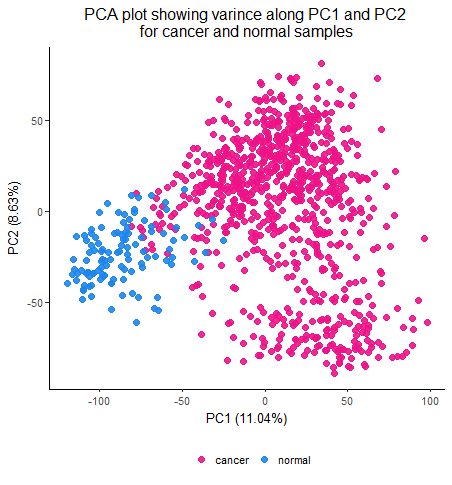
\includegraphics[scale=0.51]{pca_method.png}
            \caption{An example of PCA 2D scatter plot, showing the variance along PC1 and PC2 for cancer and normal samples.}
            \label{fig:pcamethod}
            \end{figure}
        
    \newpage
    Another way of exploring variation characterised by PCA is to visualise variation of each principal component in a series of one-dimensional (1D) box plots. Figure \ref{fig:1dpcamethod} shows the variation seen in each PC (1-9) for the cancer/normal dataset shown as a scatter plot of first two PCs in Figure \ref{fig:pcamethod}. 
    In contrast to 2D scatter plots, 1D PCA plots are able to show variation along more than two PCs at a time. This method is useful for checking if any of the other PCs contain variation worth exploring. This is useful for checking for potential presence of batch effects or signatures left by other cofactors. 
    For each PC, the variation of each condition group, here - cancer and normal, is represented by a box plot. The PCs where condition boxes have the smallest overlap (e.g. PC1) will shows the clearest separation when plotted in 2D. \\
       
    
        % PCA 1d
            \begin{figure}[h]
            \centering
            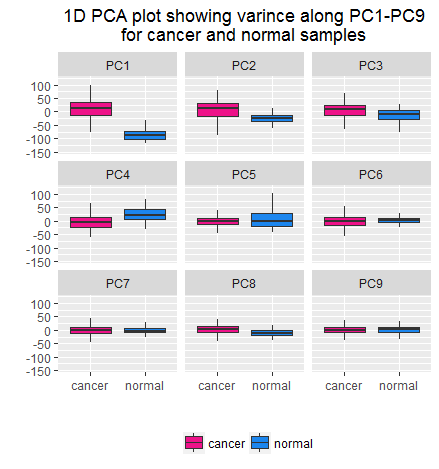
\includegraphics[scale=0.6]{1dpcamethod.png}
            \caption{An example of one-dimensional PCA plots for the cancer/normal dataset. }
            \label{fig:1dpcamethod}
            \end{figure}
   
  
    \subsection{Clustering and Heatmap representation}
    
    In clustering, or unsupervised classification, the aim is to identify subsets (clusters) in the data based on the similarity between single objects. Similar objects should be assigned to the same cluster, while objects which are not similar to each other, should be assigned to different clusters.
    Cluster analysis is applied to transcriptomics data to search for similar gene expression patterns between individual samples. This can help to reveal the data structure and give first insights into the data, which is especially useful if prior knowledge is little or non-existent. Clustering can, therefore, be seen as exploratory data analysis. 
        
    The purpose of clustering transcriptomics data is to statistically group samples according to their gene expression, in order to reduce complexity and dimensionality of the data, predict function or identify shared regulatory mechanisms \cite{Metsalu2015ClustVis:Heatmap}. Clustering can be performed as a part of heatmap. Heatmap is a datamatrix visualising values in the cells by the use of a color gradient. This gives a good overview of the largest and smallest values in the matrix. Rows (genes) and/or columns (samples) of the matrix are clustered to facilitate interpretation of sets of rows or columns rather than individual ones \cite{Metsalu2015ClustVis:Heatmap}.
    
    \newpage
    One of the popular methods is Hierarchical Clustering, which involves re-ordering of samples based on their distance in high dimensional space. The cluster is constructed based on the determination of two parameters — the distance metric and the linkage criterion. Objects close to each other in the hierarchy, measured by tracing the branch heights, are also close by some measure of distance — for example, individuals with similar expression profiles will be close together in terms of branch lengths.
    
    
    The two most common distance measures used for clustering are Euclidean and Manhattan distances. Typically the results of the two are quite similar, and most studies default to using the Euclidean measure. 
    
    The Euclidean distance involves computing the square root of square differences between two coordinates. In this way, the shortest path diagonally is calculated: $$ \sqrt{(x_{1}-x_{2})^{2}+(y_{1}-y_{2})^{2}}$$ where the first point is $(x1, y1)$ and the second point is $(x2, y2).$
    
    The Manhattan distance between two points is calculated by taking the sum of the lengths of the differences between the coordinates. Therefore, the distance is measure not in a straight line, but on horizontal (x) and vertical (y) axes: $$ (x_{1}-x_{2})+(y_{1}-y_{2})$$
    

   An example of unsupervised clustering of samples with heatmap is shown in Figure \ref{fig:heatmapmethod}. The data is clustered by columns (samples) and rows (genes), with dendograms showing how clusters are formed. The colour bar above the heatmap shows cancer/normal samples as pink/blue lines, and clustering forms blocks of colour. The heatmap colours  represent gene expression intensity according to the scale (high expression - dark blue, low expression - light yellow). 
   This example shows how cancer and normal samples form two major clusters in the dendogram, which is noticeable in the heatmap colouring as well. Some of the samples are not within the expected clusters, i.e. are outliers, but that is in agreement with the observed  slight overlap between cancer and normal samples clusters on the PCA plot (Figure \ref{fig:pcamethod}).

     % heatmap method
        \begin{figure}[h]
        \centering
        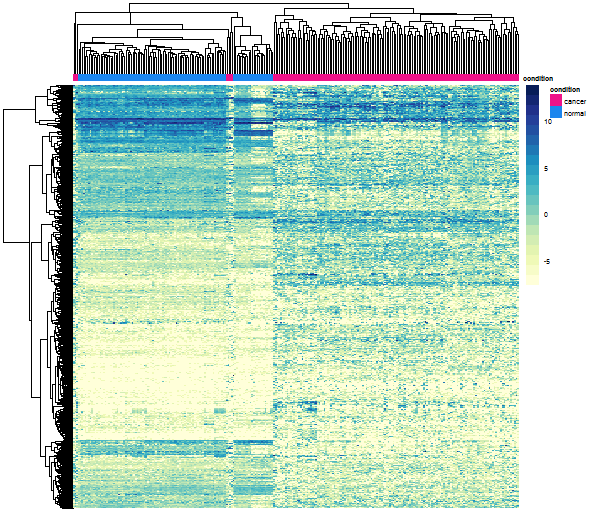
\includegraphics[scale=0.4]{heatmapmethod2.png}
        \caption{An example of clustering of the cancer/normal samples with heatmap representation. The data was clustered with Euclidean distance and average linkage. }
        \label{fig:heatmapmethod}
        \end{figure}
    
    Prior to clustering the data is normalised and filtered for low expression as described in  section \ref{}. The heatmaps were generated using Euclidean distance with average linkage (default) using the R package  \texttt{pheatmap} \cite{kolde2012pheatmap}. Clustering without heatmap representation was done with the R function \texttt{hclust()} with default parameters.


   

\newpage


\subsection{Batch effects}

Batch effects are a common and powerful source of variation in high-throughput biology.  They are artifacts not related to the biological variation of scientific interests, and may substantially affect the downstream analysis results if not dealt with properly. 
To identify the existence of batch effects, exploratory analyses must be carried out to help quantify their effect, so that downstream statistical analyses can then be adjusted to account for these unwanted effects. 
 
Batch effects are sub-groups of measurements that have qualitatively different behaviour across conditions and are unrelated to the biological variables in a study \cite{Leek2010}. For example, batch effects may occur if a subset of experiments was run on two different week days, if two technicians were responsible for different subsets of the experiments or if two different lots of reagents or instruments were used. This becomes a major problem when batch effects are correlated with an outcome of interest and lead to incorrect conclusions.
 
Although batch effects are difficult or impossible to detect in low-dimensional assays, high-throughput technologies provide enough data to detect and even remove them \cite{Leek2010}. 
 
One way to quantify the affect of non-biological variables is to examine the principal components of the data. Principal components are estimates of the most common patterns that exist across features, as discussed in the previous section. Principal components can capture both biological and technical variability and therefore can be used to quantify the effects of artifacts on the high-throughput data \cite{LeekCapturingAnalysis}. Principal components can be compared to known variables, such as sample source and time. 
 
Of more concern are cases in which batch effects are confounded with an outcome of interest and result in misleading biological or clinical conclusions \cite{Leek2010}. An example of confounding is when all of the cases are processed on one day and all of the controls are processed on another. In this project, it will be crucial to check if any of the cancer sample subgroups are linear with sample processing site or time (year sample taken). In an ideal experimental design comparing a molecular profile in tumour and healthy samples, the samples should be equally distributed between multiple laboratories and across different processing times. These steps can help to minimize the probability of confounding between biological and batch effects.
 
%this part is a bit weird
In sum, the first step in the exploratory statistical analysis of batch effects is to identify and quantify batch effects using principal components analysis or other visualization techniques. If strong batch effects exist, they must be accounted for in downstream statistical analyses. 

 


\section{Hypothesis-driven analysis methods}    




    \subsection{Differential Expression Testing}
    \subsubsection{Approach Motivation/Background}
    In RNA-seq, mapped reads are aggregated to counts at different levels, such as transcripts, exons, or genes. The counts for a given gene quantifies the expression of that gene. The main goal is to find which genes have different levels of expression under different experimental conditions –- this is known as differential expression.
    The detection of differentially expressed genes between two or more conditions is one of the most commonly asked questions biological research, and RNA-sequencing is currently the primary technology used for gene expression profiling.

    There are several tools within Bioconductor that have been developed for the differential analysis of count data, including DESeq \cite{}, DESeq2 \cite{}, edgeR \cite{Robinson2010EdgeR:Data}, limma (voom) \cite{Ritchie2015LimmaStudies}.

    The two main goals of using tools for differential expression analysis are:
    \begin{enumerate}
    \item Estimate the magnitude of differential expression between two or more conditions based on read counts from replicated samples, i.e. calculate the fold change of read counts, taking into account the differences in sequencing depth and variability.
    \item Estimate the significance of the difference and correct for multiple testing.
    \end{enumerate}

        
        \subsubsection{Limma-voom}
        \textit{limma} is an R/Bioconductor package \cite{Ritchie2015LimmaStudies, smyth2004linear}  that provides an integrated set of tools for differential expression analysis. The \textit{limma} pipeline includes linear modeling with extensive features for handling complex experimental designs with multiple treatment factors, and empirical Bayes statistical methods to borrow strength between genes to overcome the problem of small sample sizes \cite{Ritchie2015LimmaStudies}.

        The \textit{limma} approach estimates the mean-variance relationship of gene expression data in log-CPM  (log-counts normalized for sequence depth) \cite{Law2014}. The \texttt{voom()} method (an acronym for ‘variance modeling at the observational level’) incorporates the mean-variance trend into a precision weight for each individual normalised observation. The normalised log-counts and associated precision weights are then passed on to the \textit{limma} empirical Bayes analysis pipeline \cite{Law2014}.
        
        Simulation studies show that the \textit{limma-voom} performs as well or better than other count-based methods even when the data are generated according to the assumptions of the earlier methods  \cite{Law2014}. A key advantage of the \textit{limma} pipeline is that it provides accurate type I error rate control even when the number of samples in the analysis is small \cite{SmythLimma:Guide}, which is a problem for other methods. Additionally, \textit{voom} can robustly handle heterogeneous data with outliers and hypervariable genes \cite{phipson2013empirical}, and also the analysis run-time is fast, which makes it the most suitable tool for differential expression testing in this project. 
        
        \subsubsection{Linear Models}
        
        The hallmark of the \textit{limma} approach is the use of gene-wise linear models to analyse entire experiments as an integrated whole rather than simple comparisons between pairs of treatments  \cite{Ritchie2015LimmaStudies}, therefore allowing more flexible hypotheses. The effect of sharing information between samples allows one to model correlations that may exist between samples due to replication of samples or presence of covariates. This kind of information would not accessible if the data was partitioned into subsets and analysed as a series of pairwise comparisons \cite{Love2016RNA-SeqApproved}. In this way, linear models permit very general analyses, in which it is possible to adjust for the effects of multiple experimental factors or batch effects  \cite{Ritchie2015LimmaStudies}.
        
        In the linear model approach,  two matrices have to be specified. The first is the \textit{design matrix} which provides a representation of the experimental design, i.e. each column corresponds to a coefficient that describes the sample source. The second is the \textit{contrast matrix} which specifies which comparisons have to be made between the samples. In this way, linear models describe how the treatment factors are assigned to the different samples, in matrix terms: $$ E(y_g) = X \beta_g$$ where $y_g$ is the vector of log-CPM values (expression data) for a gene $g$, and $X$ is the design matrix with the $x_i $ as rows, and $ \beta_g$ is a vector of coefficients. The contrasts of interest are given by $$\alpha_j = C^T \beta_g$$ where $C$ is the contrast matrix. The coefficients component of the fitted model produced by \textit{limma} function \texttt{lmFit()} contains estimated values for the $\beta_g$. After applying \texttt{contrasts.fit()}, the coefficients component now contains estimated values for the $\alpha_j$ \cite{Smyth2005}.
        
        \subsubsection{Significance Testing}
        
        The number of differentially expressed (i.e. up- and downregulated) genes for each contrast (i.e. condition comparison) can be obtained after the linear model has been fit. Significance of differential expression is defined using an adjusted p-value cut-off and a log fold change (logFC) threshold.
        Fold change shows how much a gene’s expression level has changed between two conditions. This value is reported on a logarithmic scale to base 2: for example, a $log2$ fold change of $1.5$ means that the gene’s expression is increased by a multiplicative factor of $2^{1.5} \approx 2.82$.
        
        The results of fitting a linear model are summarised and subjected to hypothesis testing to see whether there is enough evidence to reject the null hypothesis that there is zero effect of the condition on the gene and that the observed difference between the conditions is due to experimental variability (i.e. variability expected to be between different samples in the same treatment group) \cite{Love2016RNA-SeqApproved}.
        
        The results of hypothesis testing is reported as a p-value. A p-value indicates the probability that a fold change as strong as the observed one, or even stronger, would be seen under the            situation described by the null hypothesis  \cite{Love2016RNA-SeqApproved}.  For analyses comprising a large number of hypothesis tests, as it is in differential expression studies, a large number of inferences may occur by chance, leading to falsely significant results \cite{pounds2006estimation}. As the hypothesis is tested for every comparison, the p-values need to be corrected/adjusted for multiple testing. The most popular form of adjustment is ‘FDR’ which is Benjamini and Hochberg’s method to control the false discovery rate \cite{BH1995}. The adjusted p-values satisfy the property that thresholding at a specific value defines a set of tests (one for each gene) with a bounded false discovery rate (FDR), typically a useful metric for assessing which genes to target for further analysis [??].



        \subsubsection{Application to the dataset}
        Limma-voom was used to perform differential expression (DE) analysis on the final dataset of TCGA-BRCA RNA-seq samples. The differential expression was quantified between the subgroups of the three main classification methods/effects (PAM50, stage, morphology) and the normal samples. 
        For each main effect, a separate design matrix was created and used to fit the model. All three effects were not included into one model together, as this would have resulted in non-estimable coefficients due to linear dependency of the effects. Each of the separate models included other cofactors and batch effect terms. 
        
        However, as the combination of subgroups of the main classification methods can have a unique effect in terms of differential expression, additional models with each pair of subgroups as factors were created. In this way it was possible to test DE not only between stages, but also between stages of a particular PAM50 subtype or morphology. 
        
        Differential expression results from the tested models used were filtered with significance threshold of logFC $>1$ and adjusted p-value $<0.05$. The genes declared as significantly differentially expressed were used in the enrichment analysis. 
        
        


    \newpage
    \subsection{Gene Expression Clustering}
    
 
\subsubsection{Approach Motivation/Background}
Clustering, or unsupervised classification,  is a powerful tool in gene expression data analysis, as it can help to reveal the structured expression patterns hidden in high-dimensional gene expression datasets \cite{Kumar2007Mfuzz:Data}, as already discussed in Section 2.2.2 in exploratory context. Genes showing similar expression patterns (\textit{co-expressed} genes) are often functionally related and controlled by the same regulatory mechanisms (\textit{co-regulated} genes), resulting in expression clusters frequently being enriched by genes of certain functions. This makes clustering an attractive method for using in the search for autophagy signatures. 
 
There are many clustering methods that can be applied to gene expression data, such as k-means clustering or the aforementioned hierarchical clustering. These common methods, however, produce hard partitions of the data, i.e. genes are assigned to exactly one cluster even if their expression profile is similar to several cluster patterns. For experiments where the change of expression over time is of interest, this might not be the best approach. It is known that regulation of genes is generally not in an `on-off` fashion, but rather is a gradual change which allows a more refined control of the genes' functions  \cite{Kumar2007Mfuzz:Data}. Therefore, clustering should ideally take into account this complexity and produce more flexible clusters by allowing gene assignment to several clusters.
 
This type of clustering algorithm is termed \textit{soft-clustering}, as it does not  create hard boundaries between clusters. 
 
\subsubsection{Soft-clustering}
 
The soft-clustering algorithm used in this project is implemented in R package \texttt{mfuzz} \cite{Kumar2007Mfuzz:Data}  using the fuzzy c-means algorithm (of the \texttt{e1071} package) based on the iterative optimization of an
objective function to minimize the variation of objects within clusters  \cite{Bezdek1981PatternAlgorithms}.
 
Fuzzy clustering differentiates how closely a gene follows the dominant cluster patterns and assigns it degrees of membership to a cluster. The membership value $\mu_{ij}$ can vary between zero and one, and is an indication of how well gene $i$ is represented by cluster $j$. This approach strongly contrasts hard-clustering where membership is binary (i.e. 0 or 1), and enables fuzzy clustering to provide more information about the structure of gene expression data \cite{Kumar2007Mfuzz:Data}. 
The formed clusters are visualised by the mfuzz plotting function, an example shown in Figure \ref{fig:mfuzzmethod}. 

        % mfuzz 
        \begin{figure}[!h]
        %\centering
        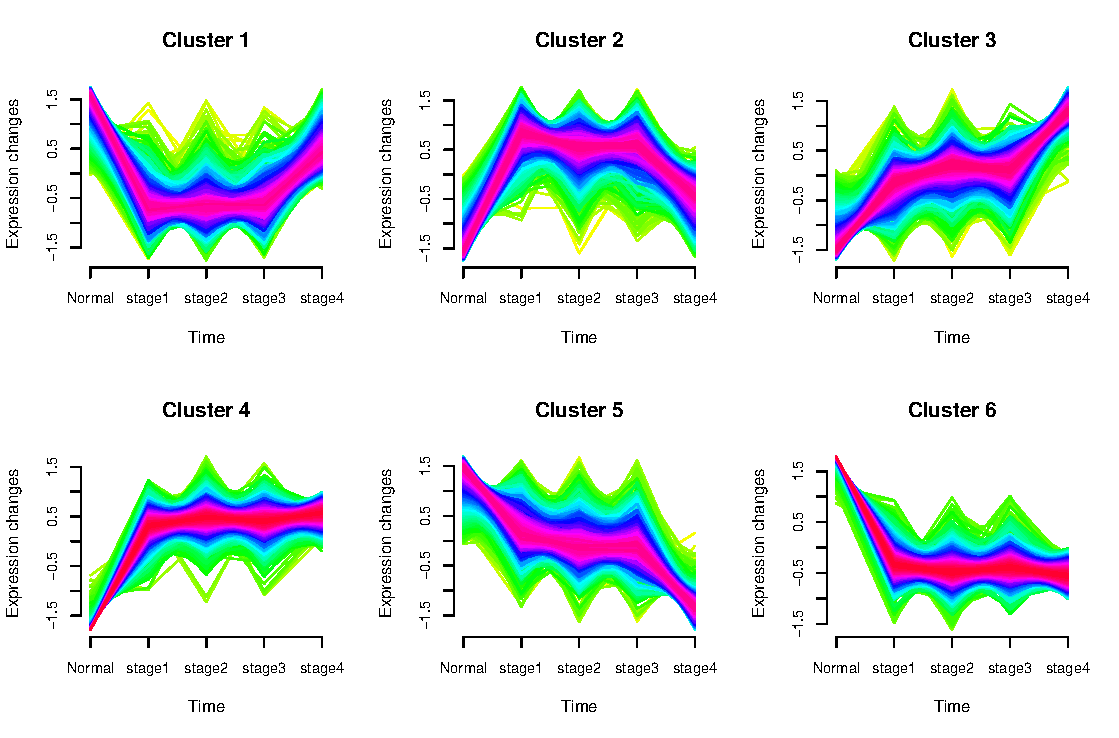
\includegraphics[width=0.75\linewidth]{mfuzzmethod.pdf}\hfill
        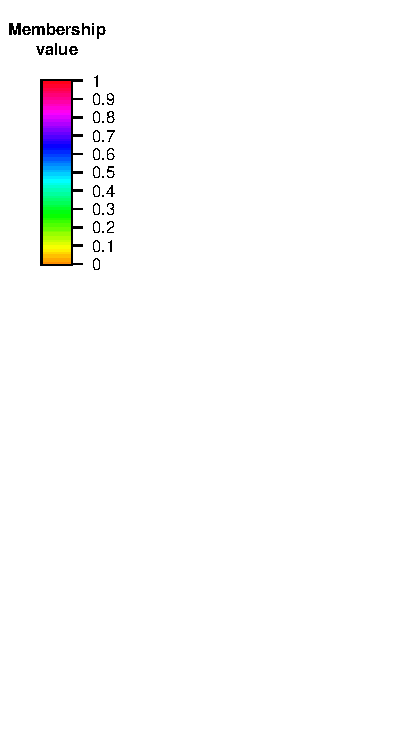
\includegraphics[width=0.2\linewidth]{mfuzzcolorbar_pad.pdf}
        \caption{An example of soft-clustering results from gene expression data. Each cluster describes an expression pattern in the dataset (y-axis), made up by genes that follow its dominant pattern across the stages (x-axis).  Green colored lines correspond to genes with low membership value; red and purple colored lines -- high membership value.}
        \label{fig:mfuzzmethod}
        \end{figure}
            
 The genes in each cluster are represented as lines color-coded by their cluster membership value.  Each cluster describes a particular expression pattern, for instance Cluster 1 comprises genes that are upregulated at all stages of cancer compared to Normal, whereas Cluster 5 shows the opposite, i.e. downregulation trend. Other, more stage-specific patterns, such as in Clusters 2 and 6 with distinct expression is Stage 4, can also be identified with this method. 
 
  
The two parameters that are specified in fuzzy clustering are the number of clusters $c$ and the fuzziness parameter $m$. The fuzziness parameter value should be chosen to minimise clustering of random data and produce maximally stable clusters. Stable clusters are usually compact and are not affected by variation of $m$, whereas weak clusters disappear if $m$ is increased \cite{Kumar2007Mfuzz:Data}. The $m$ parameter is often easiest to estimate by using the \texttt{mestimate} function specifically built for this purpose \cite{Schwammle2010AAnalysis}. 
 
  
 
The method was originally introduced for microarray data, but it is acceptable to apply it to RNA-seq data in FPKM/RPKM format \cite{Futschik2007MfuzzHomepage}.  The normalised and filtered data can be directly used in the mfuzz standardisation function prior to clustering, which scales the expression change to to zero mean and standard deviation of one (scale on y-axis).
The genes in the resulting clusters can be accessed and filtered by their membership score for inclusion in further analysis. The suggested membership score to use as a cut-off to select genes representing a particular cluster is 0.6. 

\subsubsection{Application to the dataset}

Mfuzz was used to perform soft-clustering on the gene expression data with the input set of genes being the same as for differential experssion analysis, i.e. 15874 genes. The count data was TMM-normalised and transformed to log-RPKM format. Then, \texttt{removeBatchEffect()} function from \texttt{limma} package \cite{Ritchie2015LimmaStudies} was used create expression matrix where two batch effect sources, year and sample source site, have been taken into account prior to clustering the data. 

Clustering was performed on all samples together and on individual PAM50 subtypes. For consistency, all analysis runs were done for six clusters (\textit{c})  with fuzziness parameter (\textit{m}) estimated by \texttt{mestimate} function. In each cluster, only genes with membership value of 0.6 or higher were used in the subsequent enrichment analysis. 





    \newpage
    \subsection{Enrichment Analysis}
    
    
      \subsubsection{Approach Motivation/Background}
        Gene expression analysis approaches produce lists of genes that are classified as ‘interesting’ in terms of their expression pattern (e.g. differentially expressed or clustered genes), but their immediate relevance to the study objective may be unclear. If 1,000 genes have changed in an experimental condition, it may be difficult to interpret the meaning of this change, and also one may be biased to only pay attention to the genes that are relevant to the study. 

        A solution is the use of enrichment/overrepresentation analysis, which aims to detect whether a group of objects has certain properties more (or less) frequent than can be expected by chance \cite{Goeman2007AnalyzingIssues}. In biological sense, whether a candidate set of genes appears in the list of ‘interesting’ genes more frequently than genes picked at random would. 

        A gene set is a classified groups of genes into a biologically relevant group, which can be the members of the same biochemical pathway, be annotated with the same molecular function or expressed in the same cellular compartments. In this project, the gene set is the curated list of autophagy-related genes. 
        
        For enrichment analysis, four groups of genes are defined (Figure \ref{fig:fishervenn}):
        
        \begin{itemize}
        \textit{m} is the total number of genes\\
        \textit{n} is the number of genes in a set, e.g. autophagy genes\\
        \textit{j}  is the number of ‘interesting’ genes, e.g. differentially expressed genes or genes in a cluster\\
        \textit{k} is the number of ‘interesting’ genes in the gene set\\
        \end{itemize}
        
         % fisher venn
                    \begin{figure}[!h]
                    \centering
                   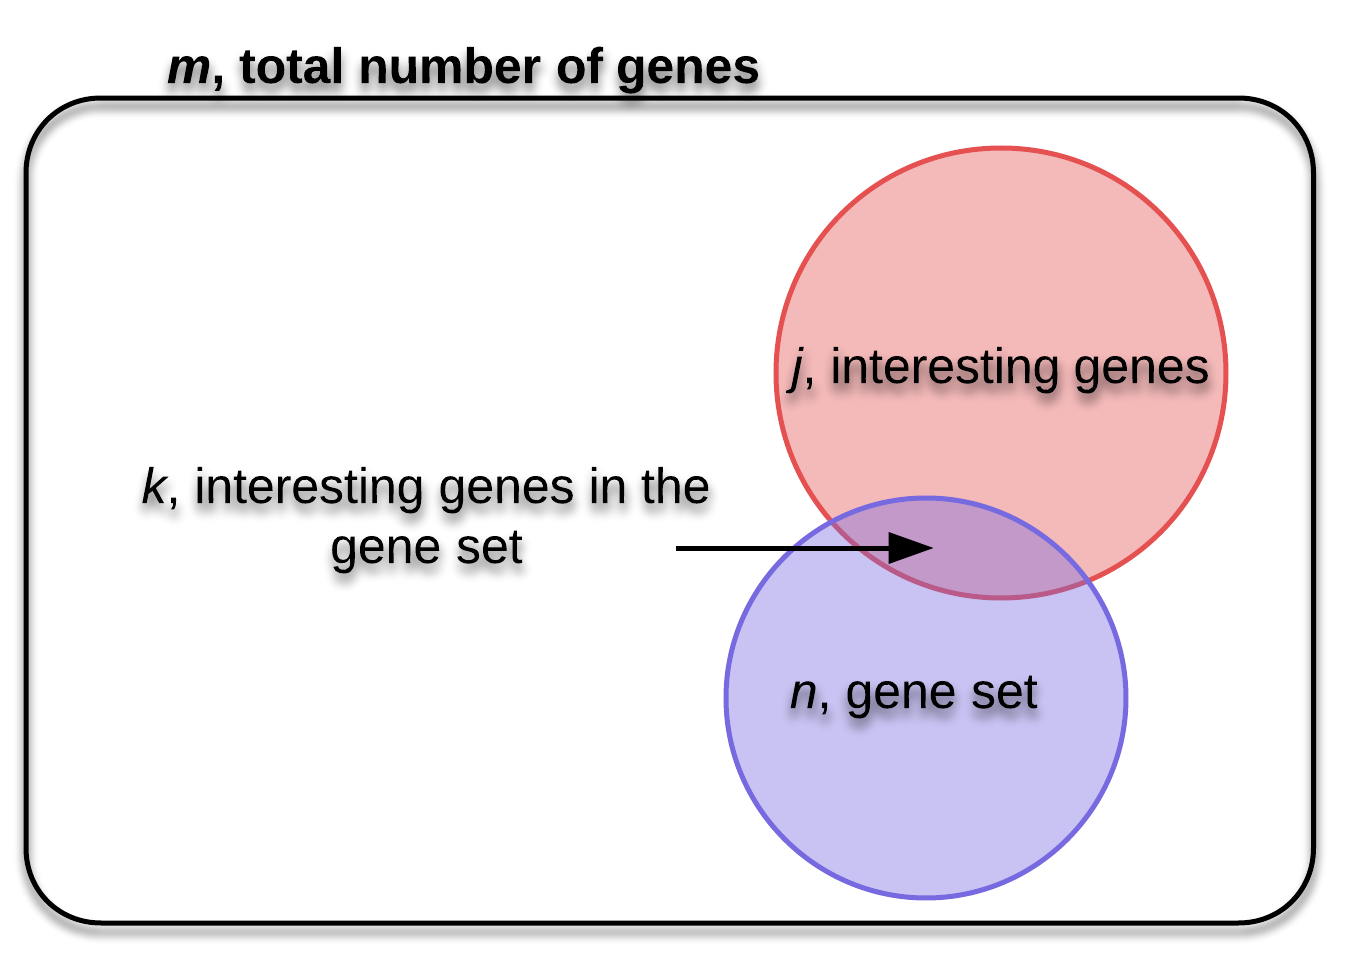
\includegraphics[scale=0.18]{fisher_venn2.png}
                    \caption{The relationships between groups of genes defined in Enrichment Analysis}
                    \label{fig:fishervenn}
                    \end{figure}
                    
        \subsubsection{Fisher's Exact Test}
        
        A common approach for performing enrichment analysis is the Fisher’s exact test. It is a statistical significance procedure for examining the association between two categorical variables \cite{Fishersexacttest}. 
        
        To answer the question of whether a gene set is enriched in the list of interesting genes, it is common to start with a \textit{2-by-2} contingency table. Table \ref{table:constable} shows the setup for a contingency table with the distribution of one variable in rows and another in columns. The character group labels (\textit{m,n,k,j}) indicate how each values is calculated. The resulting matrix is used directly in the R function \texttt{fisher.test()}. 
        
       \begin{table}[!h]
        \centering
        \caption{The set up for \textit{2-by-2} contingency table. The gene set in this project is the autophagy-related genes, and the ‘interesting’ genes can me differentially expressed genes or genes represented by a cluster.  }
        \label{table:constable}
        \begin{tabular}{c|c|c}
             & \textbf{Not interesting genes} & \textbf{Interesting genes} \\ \hline
            \textbf{\begin{tabular}[c]{@{}c@{}}Other\\  genes\end{tabular}} & \textit{m-n-j+k} & \textit{j-k} \\ \hline
            \textbf{\begin{tabular}[c]{@{}c@{}}Gene set\\  genes\end{tabular}} & \textit{n-k} & \textit{k}
            \end{tabular}
        \end{table}
        

        \newpage
        The null hypothesis of the Fisher's test assumes that the variables are independent and the sums of columns and rows are  fixed\cite{Goeman2007AnalyzingIssues}. Consequently, the values in contingency table are used to calculate the probability that this or any table with more extreme joint values (unobserved) would occur under the null hypothesis \cite{PathwayGuide.}. The calculated probabilities are expressed as p-values, and a small p-value indicates a discrepancy between the data and the null hypothesis of no association between variables.
        
        In addition to p-value, \texttt{fisher.test()} also returns an \textit{odds-ratio}, which is the ratio between proportions in and outside the sample. In other words, it is a measure of the magnitude of the difference. When testing for enrichment, the upper tail of the distribution, which means that a one-sided test is performed. A two-sided test would imply also testing the the lower tail of the distribution, so testing for depletion.


        \subsubsection{Application to the dataset}
        
        
        Enrichment analysis was carried out on the results of differential expression testing to check whether autophagy-related genes are enriched among the DE genes in any of the model contrasts. The Fisher's test was performed on all DE genes, and also on up- or downregulated separately. As three individual gene sets, all autophagy genes, only autophagy core genes, and only autophagy-related transcription factors were used. 
        The same enrichment analysis set-up was applied to the soft-clustering results. Genes in separate clusters with membership value of at least $0.6$ were tested for enrichment of the gene sets.

        The significance of autophagy enrichment was defined by odds-ratio 
        $>1$, and FDR-adjusted p-value $>0.05$. 




        %for results/disc:
        % High level understanding of the biology behind gene expression – Interpretation!·
        % Translating changes of hundreds/thousands of differentially expressed genes into a few biological processes (reducing dimensionality)

    
